\chapter{Выполнение лабораторной работы}

\section{Цель работы}

Лабораторная работа № 2 нацелена на освоение возможностей программы Microsoft Project для работы с ресурсами.

\section{Тестовое задание}

Добавить в тестовое задание лабораторной работы № 1 информацию о ресурсах, представленных сотрудниками с стандартной ставкой 250 руб/день, фиксированной выплатой в 5000 рублей и ресурсом со ставкой 1000 руб/нед добавляемым к работам A, B, C со второй недели реализации проекта. Распределение сотрудников по работам представлено в таблице~\ref{tab:tz1}.
\begin{table}[H]
\caption{Ресурсы проекта тестового задания}
\label{tab:tz1}
\centering
\begin{tabular}{|c|c|}\hline
	Название работы & Количество исполнителей (чел.) \\
	\hline
	Работа A & 1\\
	\hline
	Работа B & 4 \\
	\hline
	Работа C & 5\\
	\hline
	Работа D & 2\\\hline
	Работа E & 3\\\hline
	Работа F & 3\\\hline
	Работа G & 5\\\hline
	Работа H & 5\\\hline
	Работа I & 2\\\hline
	Работа J & 6\\\hline
\end{tabular}
\end{table}

Созданный список ресурсов представлен на рисунке~\ref{fig:res1}.

\begin{figure}[H]
	\centering
	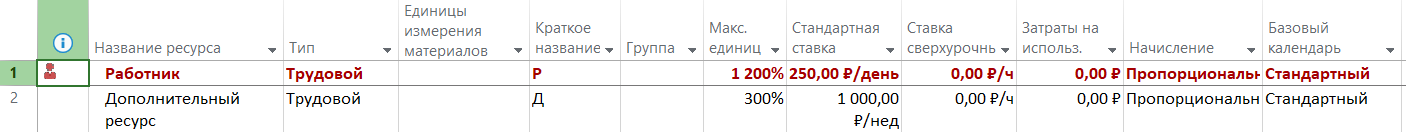
\includegraphics[width=\linewidth]{images/test_res_list.png}
	\caption{Список ресурсов}
	\label{fig:res1}
\end{figure}

Список работ с назначенными ресурсами представлен на рисунке~\ref{fig:res2}.

\begin{figure}[H]
	\centering
	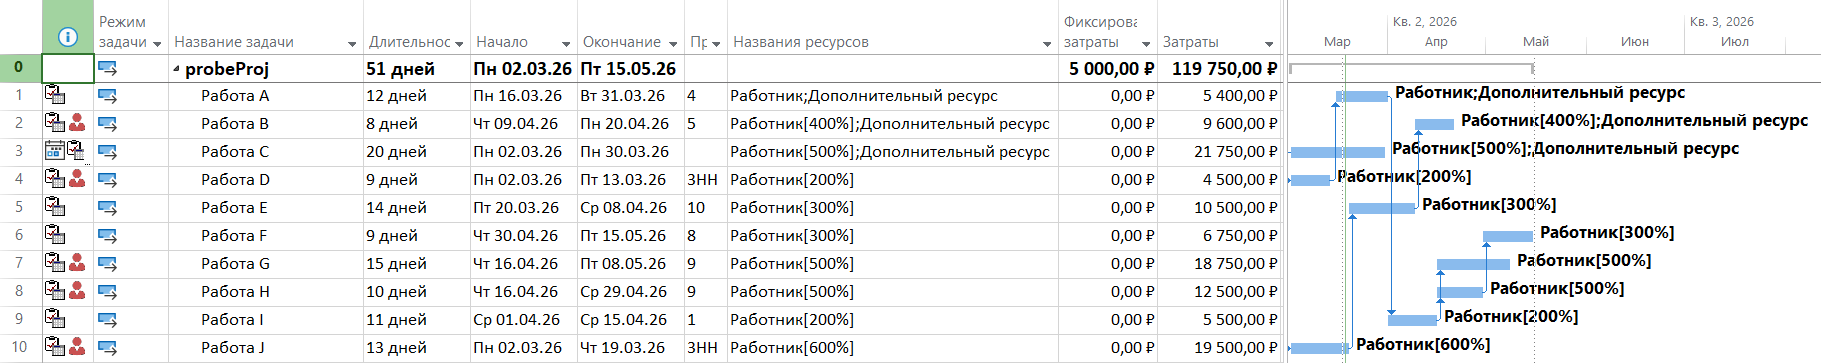
\includegraphics[width=\linewidth]{images/res_task_list_with_res.png}
	\caption{Список работ с назначенными ресурсами}
	\label{fig:res2}
\end{figure}

Ввозникает перегрузка ресурса работников на некоторых задачах.

% \imgs{test-result}{h!}{0.3}{Результат выполнения тестового задания}


\section{Краткое описание проекта}

Команда разработчиков из 16 человек занимается созданием карты города на основе собственного модуля отображения. Проект должен быть завершен в течение 6 месяцев. Бюджет проекта: 50 000 рублей.

\section{Задание 1}

Создать список ресурсов.

На рисунке~\ref{fig:sved} представлен список ресурсов проекта.
\begin{figure}[H]
	\centering
	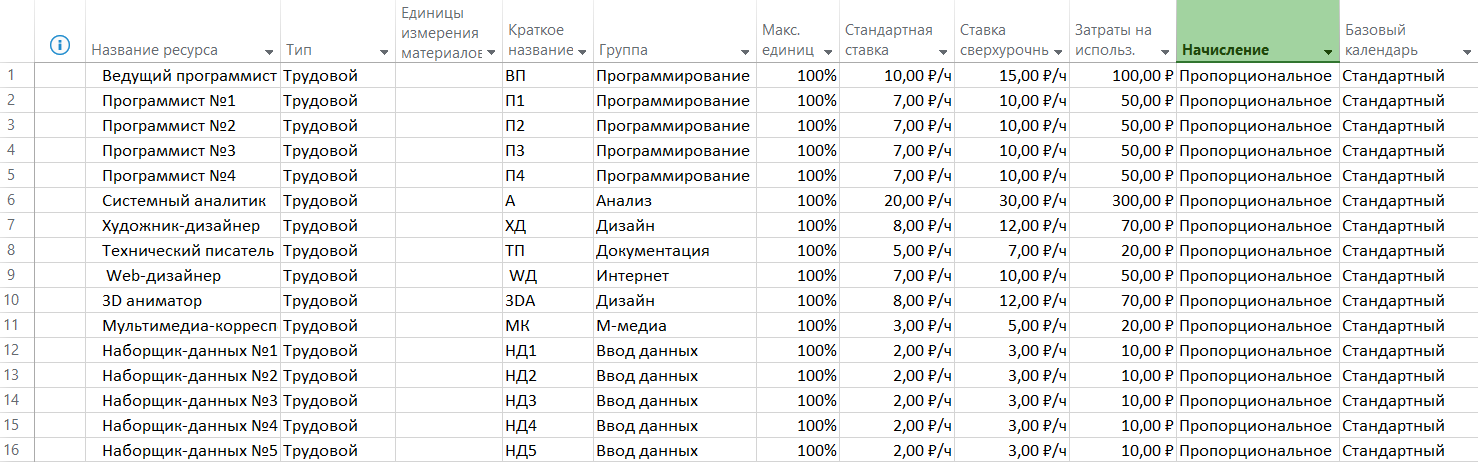
\includegraphics[width=\linewidth]{images/step1_resource_list.png}
	\caption{Ресурсы проекта}
	\label{fig:sved}
\end{figure}

\section{Задание 2}

Назначить ресурсы задачам.

На рисунке~\ref{fig:schedule} представлен список задач с назначенными ресурсами.
%	\imgs{task1-2}{h!}{0.5}{Параметры проекта}
\begin{figure}[H]
	\centering
	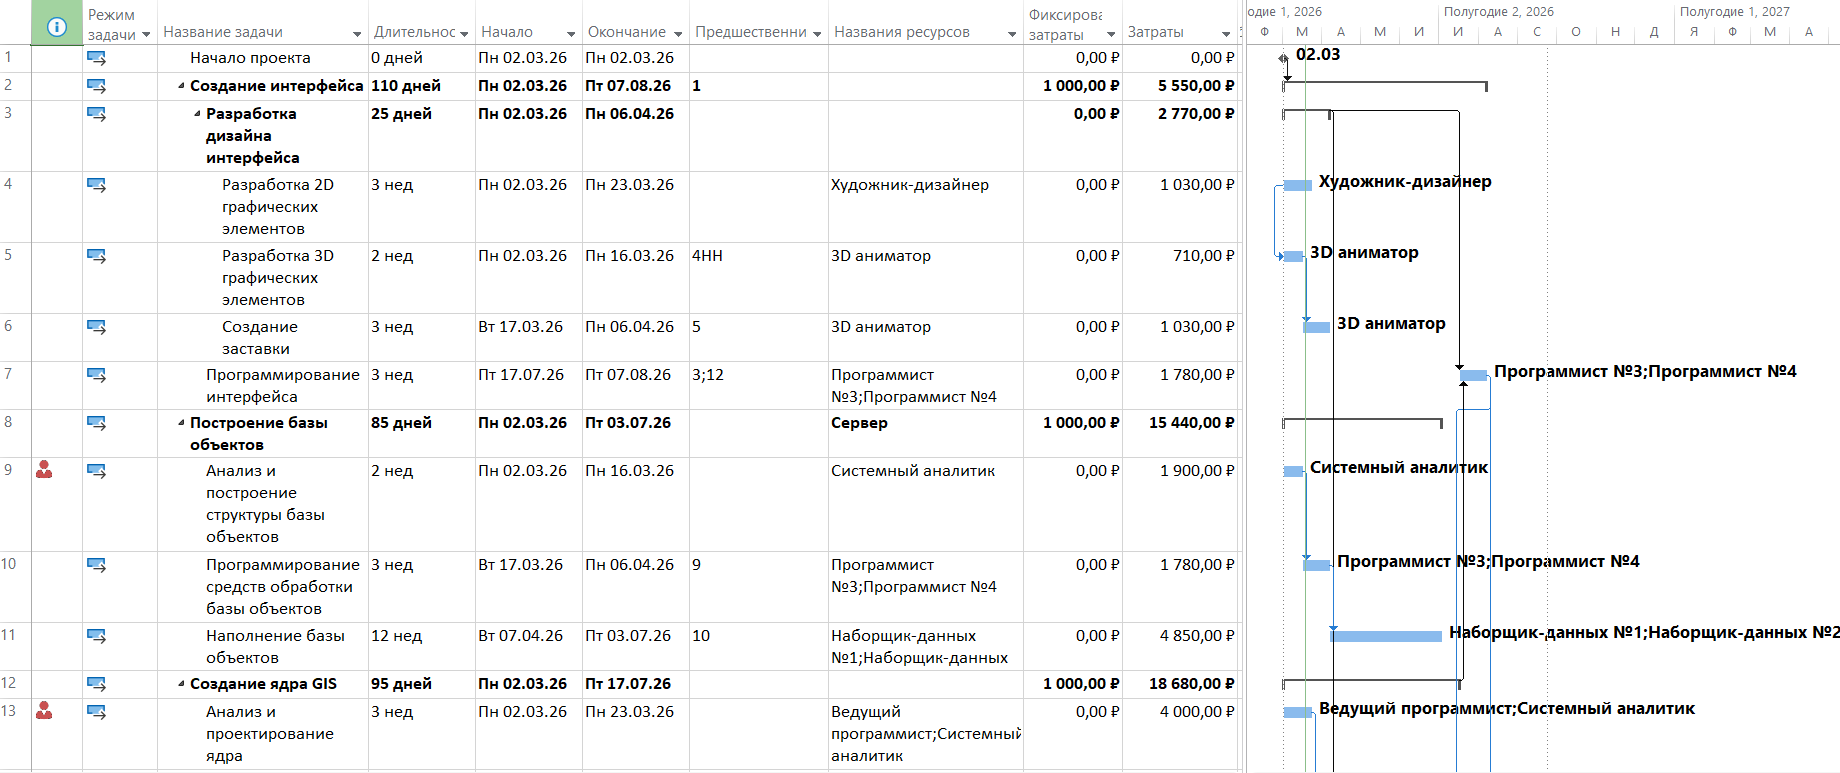
\includegraphics[width=\linewidth]{images/task_with_resources.png}
	\caption{Список задач с назначенными ресурсами}
	\label{fig:schedule}
\end{figure}

Аренда сервера была выделена отдельным ресурсом с круглосуточной работой и ставкой 2 руб/час.

Аналогично тестовому заданию возникла перегрузка для системного аналитика, технического писателя и художника-дизайнер, в связи с одновременным выполнением ими нескольких работ.

\section{Задание 3}

Проанализировать затраты по группам ресурсов.

На рисунке~\ref{fig:notes} приведена группировка ресурсов с отображением затрат и трудозатрат на группу.
%	\imgs{task1-4}{h!}{0.5}{Суммарная задача проекта и <<Заметки>>}
\begin{figure}[H]
	\centering
	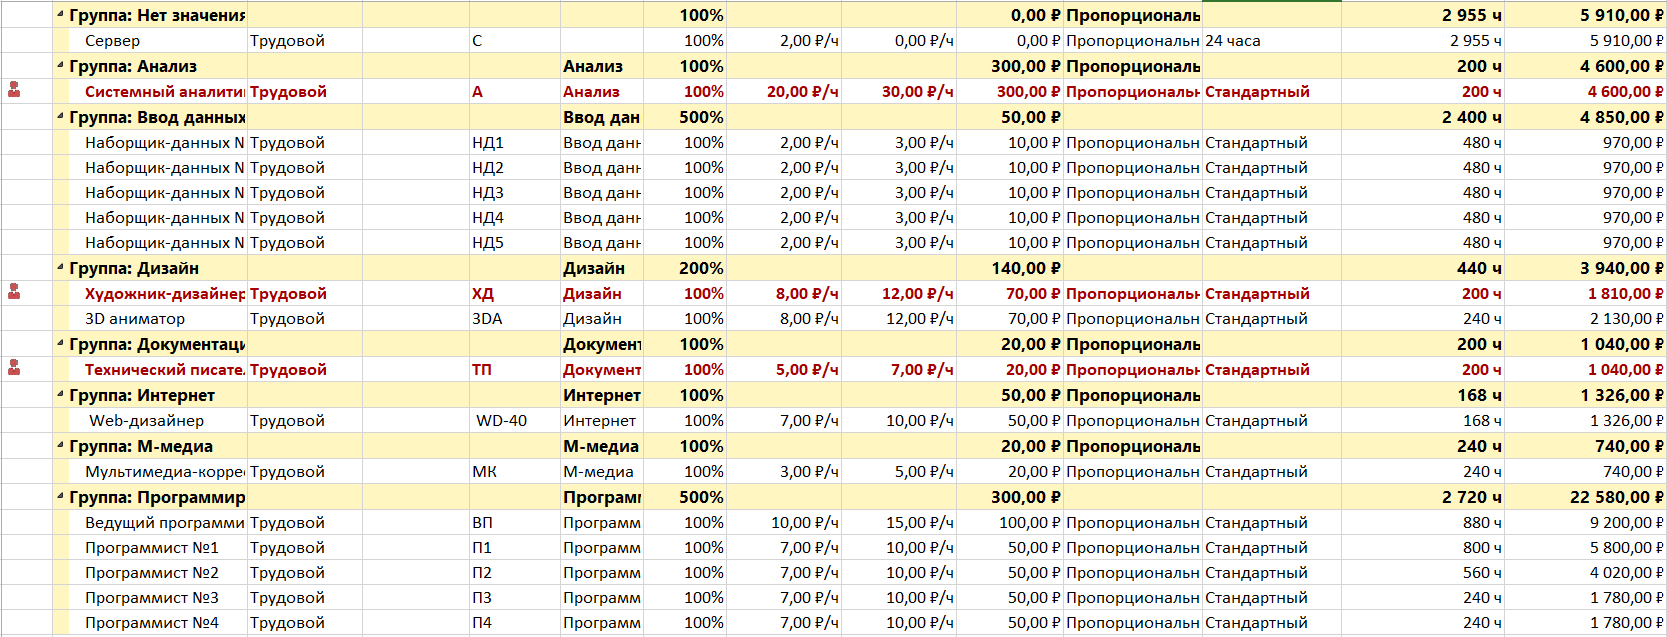
\includegraphics[width=\linewidth]{images/groupped_by_group_resources.png}
	\caption{Сгруппированные ресурсы}
	\label{fig:notes}
\end{figure}

На рисунках~\ref{fig:trudpie} и~\ref{fig:wastedpie} приведены круговые диаграммы по группам ресурсов для трудозатрат и затрат соответственно.

\begin{figure}
	\centering
	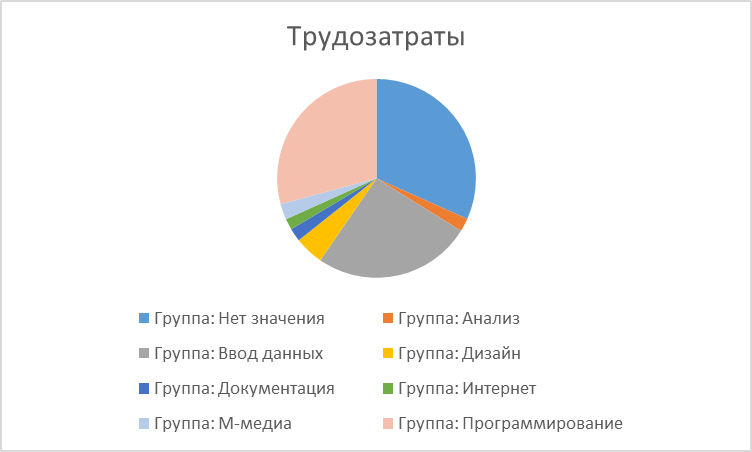
\includegraphics[width=1\linewidth]{images/trud_pie}
	\caption{Трудозатраты по группам ресурсов}
	\label{fig:trudpie}
\end{figure}
\begin{figure}
	\centering
	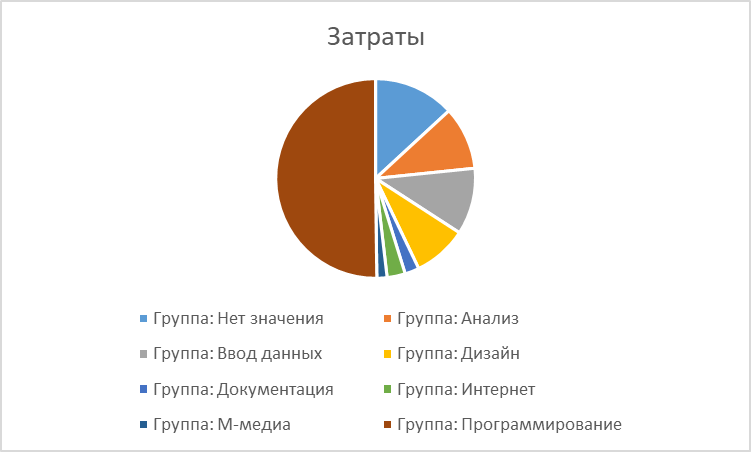
\includegraphics[width=1\linewidth]{images/wasted_pie}
	\caption{Затраты по группам ресурсов}
	\label{fig:wastedpie}
\end{figure}


\section*{Выводы}

По результатам анализа были сделаны следующие выводы:

\begin{itemize}
	\item в проекте возникают перегрузки для системного аналитика, художника-дизайнера и технического писателя в связи с необходимостью выполнения ими одновременно нескольких задач;
	\item затраты на выполнение проекта составляют 47986 руб., что не превосходит бюджета проекта в 50000 руб.;
	\item трудозатраты проекта составляют 9323 ч;
	\item затраты на работу программистов составляют около 50\% при трудозатратах, составляющих около 30\% от всех трудозатрат проекта;
	\item затраты на работу системного аналитика составляют 9,6\%, при трудозатратах составляющих 2\% всех трудозатрат проекта;
	\item затраты на аренду сервера составляют 12\% всех завтрат проекта.
\end{itemize}